%
% 1-fundamtenallemma.tex
%
% (c) 2023 Prof Dr Andreas Müller
%

%
% Integration
%
\subsection{Partielle Integration
\label{buch:felder:subsection:partint}}
Die partielle Integration für ein Integral einer Variablen
transformiert das Integral
\[
\int_{a}^{b} f(x) g'(x)\,dx
\]
in die Summe
\[
\biggl[ f(x) g(x) \biggr]_a^b
-
\int_a^b f'(x) g(x)\,dx.
\]
Der erste Term hängt nur von Informationen auf dem Rand des 
Definitionsbereichs ab.
Eine Verallgemeinerung dieser Regel muss vor allem auch klären,
wie dieser erste Term aussehen soll.
Er darf nur von den Funktionswerten der Funktionen auf dem Rand
$\partial\Omega$ abhängen.
Die Abhängigkeit muss ausserdem linear sein.
In diesem Abschnitt sollen in einer Folge von Beispielen die
wichtigsten Fälle systematisch entwickelt werden.

%
% Ableitung von Produkten
%
\subsubsection{Ableitung von Produkten}
Die Regel für die partielle Integration von Produkten von Funktionen
einer Variable ist die Integralform der Produktregel
\[
\frac{d}{dx}(f(x)g(x)) = f'(x)g(x) + f(x)g'(x).
\]
Für eine Erweiterung auf ist daher als erstes zu klären, welche Art
von Differentialoperatoren überhaupt in Frage kommen.

Die partielle Ableitung nach einer der Variablen bei Funktionen
$f$ und $g$ von $n$ Variablen erfüllt eine Produktregel:
\[
\frac{\partial}{\partial x_k}
(f(x)g(x))
=
\frac{\partial f}{\partial x_k}(x)\,g(x)
+
f(x)
\,
\frac{\partial g}{\partial x_k}(x)
\]
für jedes $k=1,\dots,n$.
Die partiellen Ableitungen sind aber nur von untergeordnetem Interesse,
da sie für sich allein von der Wahl des Koordinatensystems abhängig 
sind und daher zum Beispiel keine koordinatenunabhängige physikalische
Bedeutung haben können.

Der Gradient wurde aus der Richtungsableitung konstruiert und es wurde
gezeigt, dass 
\[
\operatorname{grad} f(x)
=
\renewcommand{\arraystretch}{1.7}
\begin{pmatrix}
\displaystyle
\frac{\partial f}{\partial x_1}\\
\vdots\\
\displaystyle
\frac{\partial f}{\partial x_n}
\end{pmatrix}
\]
eine koordinatenunabhängige Bedeutung als der Vektor hat, in dessen
Richtung die schnellste Zunahme der Funktion $f$ erfolgt.
Und tatsächlich gilt auch für den Gradienten eine Produktformel:
\begin{align*}
\renewcommand{\arraystretch}{1.7}
\operatorname{grad}(f(x)g(x))
&=
\begin{pmatrix}
\displaystyle
\frac{\partial}{\partial x_1}(f(x)g(x))\\
\vdots\\
\displaystyle
\frac{\partial}{\partial x_n}(f(x)g(x))
\end{pmatrix}
=
\begin{pmatrix}
\displaystyle
\frac{\partial f}{\partial x_1} g(x)
+
f(x) \frac{\partial g}{\partial x_1}\\
\vdots\\
\displaystyle
\frac{\partial f}{\partial x_n} g(x)
+
f(x) \frac{\partial g}{\partial x_n}
\end{pmatrix}
\\
&=
(\operatorname{grad}f(x)) g(x)
+
f(x)(\operatorname{grad}g(x))
\end{align*}
Wir haben also den folgenden Satz hergeleitet.

\begin{satz}[Produktformel für den Gradienten]
Sind $f$ und $g$ Funktionen $\mathbb{R}^n \to\mathbb{R}$, dann gilt
\[
\grad (fg) = (\grad f)g + f\grad g.
\]
\end{satz}

%
% Divergenz
%
\subsubsection{Divergenz}
Der Gradient einer Funktion $f\colon\mathbb{R}^n\to\mathbb{R}$ ist
ein sogenanntes Vektorfeld im Sinne der folgenden Definition.

\begin{definition}[Vektorfeld]
\label{buch:felder:fundamentallemma:def:vektorfeld}
Eine Abbildung $g\colon\mathbb{R}^n\to\mathbb{R}^k$, die jedem Punkt
von $\mathbb{R}^n$ einen $k$-dimensionalen Vektor zuordnet, heisst
ein {\em $k$-dimensionales Vektorfeld}.
\index{Vektorfeld}
\end{definition}

Auch für ein Vektorfeld lassen sich interessante Differentialoperatoren
definieren, deren Bedeutung später klar werden wird.

\begin{definition}[Divergenz]
\label{buch:felder:fundamentallemme:def:divergenz}
Die {\em Divergenz} eines $n$-dimensionalen differenzierbaren
Vektorfeldes $g\colon:\mathbb{R}^n\to\mathbb{R}^n$ ist die Funktion
\[
\operatorname{div} g
\colon
\mathbb{R}^n\to\mathbb{R}
:
x \mapsto
\frac{\partial g_1}{\partial x_1}(x)
+\ldots+
\frac{\partial g_n}{\partial x_n}(x)
=
\sum_{i=1}^n
\frac{\partial g_i}{\partial x_i}(x).
\]
\end{definition}

Auch für die Divergenz gibt es eine Produktformel.
Seien
\[
f\colon\mathbb{R}^3\to\mathbb{R}
\qquad\text{und}\qquad
g\colon\mathbb{R}^3\to\mathbb{R}^3
\]
stetig differenzierbare Funktionen.
Die Komponenten von $g$ schreiben wir $g_i$, $i=1,\dots,n$.

\begin{satz}[Produktformel für Divergenz]
Für eine offene Menge $U\subset\mathbb{R}^n$und
eine skalare Funktion $f\colon U\to\mathbb{R}$ und
eine vektorwertige Funktion $g\colon U\to\mathbb{R}^n$ gilt
\[
\operatorname{div}(fg)
=
\grad f \cdot g
+
f\operatorname{div}g.
\]
\end{satz}

\begin{proof}
Wir berechnen die Divergenz von $f\cdot g$:
\begin{align*}
\operatorname{div} fg(x)
&=
\frac{\partial}{\partial x_1}(f(x)g_1(x))
+
\ldots
+
\frac{\partial}{\partial x_n}(f(x)g_n(x))
\\
&=
\frac{\partial f}{\partial x_1}(x)g_1(x)
+f(x)\frac{\partial g_1}{\partial x_1}(x)
+
\ldots
+
\frac{\partial f}{\partial x_n}(x)g_n(x)
+f(x)\frac{\partial g_n}{\partial x_n}(x)
\\
&=
\sum_{i=1}^n \frac{\partial f}{\partial x_i}(x) g_i(x)
+
f(x)
\sum_{i=1}^n \frac{\partial g_i}{\partial x_i}(x)
\\
&=
\grad f(x)\cdot \operatorname{div} g(x)
+
f(x)\operatorname{div}g(x).
\qedhere
\end{align*}
\end{proof}

Die Produktregel sagt also auch hier, dass der Differentialoperator
auf jeden Faktor einzeln angewendet werden kann. 
Je nach Art des Faktors passt aber der Gradient oder die Divergenz.

%
% Laplace-Operator
%
\subsubsection{Laplace-Operator}
Besonderes Interesse an der Divergenz entsteht aus dem Zusammenhang
mit dem Laplace-Operator.

\begin{definition}[Laplace-Operator]
\label{buch:fundamentallemma:definition:laplace-operator}
Für eine zweimal stetig differenzierbare Funktion
$f\colon\mathbb{R}^n\to\mathbb{R}$
ist der {\em Laplace-Operator} definiert durch
\[
\Delta f(x)
=
\frac{\partial^2 f}{\partial x_1^2}(x)
+\ldots+
\frac{\partial^2 f}{\partial x_n^2}(x)
=
\sum_{i=1}^n \frac{\partial^2 f}{\partial x_i^2}(x).
\]
\end{definition}

Der Laplace-Operator ist ein Differentialoperator zweiter Ordnung.
Wir berechnen die Zusammensetzung der beiden Differentialoperatorn
erster Ordnung $\operatorname{div}$ und $\grad$
für eine zweimal stetig differenzierbare Funktion
$f\colon\mathbb{R}^n\to\mathbb{R}$ und erhalten
\begin{align*}
\operatorname{div}\grad f(x)
&=
\sum_{i=1}^n
\frac{\partial}{\partial x_i}
\frac{\partial f}{\partial x_i}(x)
=
\frac{\partial^2 f}{\partial x_i^2}(x)
=
\Delta f(x).
\end{align*}
Daraus lässt sich jetzt auch eine Produktformel für den Laplace-Operator
ableiten.
Dazu wenden wir ihn auf das Produkt zweier skalarer Funktionen
$f,g\colon\mathbb{R}^n\to\mathbb{R}$ an:
\begin{align}
\operatorname{div}\grad (fg)(x)
&=
\operatorname{div}\bigl((\grad f(x)) g(x) + f(x)\grad g(x)\bigr)
\intertext{nach der Produktformel für den Gradienten.
Auf die einzelnen Summanden wenden wir jetzt die Produktformel für
die Divergenz an und erhalten}
&=
(\operatorname{div}\grad f(x))g(x) + \grad f(x)\cdot \grad g(x)
\notag
\\
&\qquad\qquad
+
\grad f(x)\cdot\grad g(x) + f(x) \operatorname{div}\grad g(x).
\notag
\intertext{Durch Anwendung der Definition des Laplace-Operators
erhalten wir die gesuchte Produktformel}
\Delta (fg)(x)
&=
(\Delta f(x)) g(x) + 2\grad f(x)\cdot \grad g(x) + f(x)\Delta g(x).
\label{buch:felder:fundamentallemma:eqn:laplaceproduktformel}
\end{align}
Da der Laplace-Operator ein Operator zweiter Ordnung ist, ähnelt 
die rechte Seite von
\eqref{buch:felder:fundamentallemma:eqn:laplaceproduktformel}
der binomischen Formel.

%
% Rotation
%
\subsubsection{Rotation}
In drei Dimensionen gibt es einen weiteren interessanten Differentialoperator,
dessen Konstruktion auf dem Vektorprodukt beruht.

\begin{definition}[Rotation]
Sei $g\colon\mathbb{R}^3\to\mathbb{R}^3$ ein differenzierbares
dreidimensionales Vektorfeld, dann heisst das Vektor
\[
\operatorname{rot}g(x)
=
{\renewcommand{\arraystretch}{1.9}
\begin{pmatrix}
\displaystyle
\frac{\partial g_3}{\partial x_2}
-
\frac{\partial g_2}{\partial x_3}
\\
\displaystyle
\frac{\partial g_1}{\partial x_3}
-
\frac{\partial g_3}{\partial x_1}
\\
\displaystyle
\frac{\partial g_2}{\partial x_1}
-
\frac{\partial g_1}{\partial x_2}
\end{pmatrix}}
\]
die {\em Rotation} von $g(x)$.
\end{definition}

Die Rotation $\operatorname{rot}g$ wird im englischen Sprachraum manchmal
auch $\operatorname{curl}g$ geschrieben.
Auch für die Rotation gibt es Produktformeln für die Ableitung.

\begin{satz}[Produktformeln für die Rotation]
\label{buch:felder:fundamentallemma:satz:rotprodukt}
Für $U\subset\mathbb{R}^3$ und eine skalare differenzierbare Funktion
$f\colon U\to\mathbb{R}$ und zwei differenzierbare dreidimensionale
Vektorfelder $g,h\colon U\to\mathbb{R}^3$ gilt
\begin{align*}
\operatorname{rot}(fg)(x)
&=
(\grad f(x))\times g(x) + f(x)\operatorname{rot}g(x).
&&x\in U
\\
\operatorname{rot}(g\times h)
&=
g\operatorname{div}h
-
h\operatorname{div}g
+
(h\grad)g
-
(g\grad)h,
\end{align*}
wobei der Vektorgrand $(g\grad)h$ als $k$-te Komponente
\[
\sum_{i=1}^3 g_i\frac{\partial h_k}{\partial x_i}
=
\biggl(
\sum_{i=1}^3 g_i\frac{\partial}{\partial x_i}
\biggr)h_k
\]
hat.
\end{satz}

\begin{proof}
Der Beweis erfolgt durch Nachrechnen:
\bgroup
\renewcommand{\arraystretch}{1.9}
\begin{align*}
\operatorname{rot}(fg)
&=
\begin{pmatrix}
\displaystyle
\frac{\partial}{\partial x_2}(fg_3)-\frac{\partial}{\partial x_3}(fg_2)
\\
\displaystyle
\frac{\partial}{\partial x_3}(fg_1)-\frac{\partial}{\partial x_1}(fg_3)
\\
\displaystyle
\frac{\partial}{\partial x_1}(fg_2)-\frac{\partial}{\partial x_2}(fg_1)
\end{pmatrix}
\\
&=
\begin{pmatrix}
\displaystyle
\frac{\partial f}{\partial x_2}g_3
-\frac{\partial f}{\partial x_3}g_2
+
f\biggl(\frac{\partial g_3}{\partial x_2}
-\frac{\partial g_2}{\partial x_3}\biggr)
\\
\displaystyle
\frac{\partial f}{\partial x_3}g_1
-\frac{\partial f}{\partial x_1}g_3
+
f\biggl(\frac{\partial g_1}{\partial x_3}
-\frac{\partial g_3}{\partial x_1}\biggr)
\\
\displaystyle
\frac{\partial f}{\partial x_1}g_2
-\frac{\partial f}{\partial x_2}g_1
+
f\biggl(\frac{\partial g_2}{\partial x_1}
-\frac{\partial g_1}{\partial x_2}\biggr)
\end{pmatrix}
\\[5pt]
&=
(\grad f)\times g + f\operatorname{rot}g.
\end{align*}
\egroup
Für die zweite Identität rechnen wir
\begin{align*}
\operatorname{rot}(g\times h)
&=
\operatorname{rot}
\begin{pmatrix}
g_2h_3-g_3h_2\\
g_3h_1-g_1h_3\\
g_1h_2-g_2h_1
\end{pmatrix}
\\
&=
{\renewcommand{\arraystretch}{1.9}
\begin{pmatrix}
\displaystyle
\frac{\partial}{\partial x_2}
\bigl(g_1h_2-g_2h_1\bigr)
-
\frac{\partial}{\partial x_3}
\bigl(g_3h_1-g_1h_3\bigr)
\\
\displaystyle
\frac{\partial}{\partial x_3}
\bigl(g_2h_3-g_3h_2\bigr)
-
\frac{\partial}{\partial x_1}
\bigl(g_1h_2-g_2h_1\bigr)
\\
\displaystyle
\frac{\partial}{\partial x_1}
\bigl(g_3h_1-g_1h_3\bigr)
-
\frac{\partial}{\partial x_2}
\bigl(g_2h_3-g_3h_2\bigr)
\end{pmatrix}}
\\
&=
{\renewcommand{\arraystretch}{1.9}
\begin{pmatrix}
\displaystyle
{\color{darkgreen}
\frac{\partial g_1}{\partial x_2} h_2
}
+
{\color{darkred}
g_1 \frac{\partial h_2}{\partial x_2}
}
-
{\color{blue}
\frac{\partial g_2}{\partial x_2}h_1
}
-
{\color{orange}
g_2\frac{\partial h_1}{\partial x_2}
}
-
{\color{blue}
\frac{\partial g_3}{\partial x_3}h_1
}
-
{\color{orange}
g_3\frac{\partial h_1}{\partial x_3}
}
+
{\color{darkgreen}
\frac{\partial g_1}{\partial x_3}h_3
}
+
{\color{darkred}
g_1\frac{\partial h_3}{\partial x_3}
}
\\
\displaystyle
{\color{darkgreen}
\frac{\partial g_2}{\partial x_3}h_3
}
+
{\color{darkred}
g_2\frac{\partial h_3}{\partial x_3}
}
-
{\color{blue}
\frac{\partial g_3}{\partial x_3}h_2
}
-
{\color{orange}
g_3\frac{\partial h_2}{\partial x_3}
}
-
{\color{blue}
\frac{\partial g_1}{\partial x_1}h_2
}
-
{\color{orange}
g_1\frac{\partial h_2}{\partial x_1}
}
+
{\color{darkgreen}
\frac{\partial g_2}{\partial x_1}h_1
}
+
{\color{darkred}
g_2\frac{\partial h_1}{\partial x_1}
}
\\
\displaystyle
{\color{darkgreen}
\frac{\partial g_3}{\partial x_1}h_1
}
+
{\color{darkred}
g_3\frac{\partial h_1}{\partial x_1}
}
-
{\color{blue}
\frac{\partial g_1}{\partial x_1}h_3
}
-
{\color{orange}
g_1\frac{\partial h_3}{\partial x_1}
}
-
{\color{blue}
\frac{\partial g_2}{\partial x_2}h_3
}
-
{\color{orange}
g_2\frac{\partial h_3}{\partial x_2}
}
+
{\color{darkgreen}
\frac{\partial g_3}{\partial x_2}h_2
}
+
{\color{darkred}
g_3\frac{\partial h_2}{\partial x_2}
}
\end{pmatrix}}
\\
&=
{\color{darkred}
g\operatorname{div}h
}
-
{\color{blue}
h\operatorname{div}g
}
+
{\renewcommand{\arraystretch}{1.9}
\begin{pmatrix}
\displaystyle
{\color{blue}
h_1\frac{\partial g_1}{\partial x_1}
}
+
{\color{darkgreen}
h_2\frac{\partial g_1}{\partial x_2}
}
+
{\color{darkgreen}
h_3\frac{\partial g_1}{\partial x_3}
}
\\
\displaystyle
{\color{darkgreen}
h_1\frac{\partial g_2}{\partial x_1}
}
+
{\color{blue}
h_2\frac{\partial g_2}{\partial x_2}
}
+
{\color{darkgreen}
h_3\frac{\partial g_2}{\partial x_3}
}
\\
\displaystyle
{\color{darkgreen}
h_1\frac{\partial g_3}{\partial x_1}
}
+
{\color{darkgreen}
h_2\frac{\partial g_3}{\partial x_2}
}
+
{\color{blue}
h_3\frac{\partial g_3}{\partial x_3}
}
\end{pmatrix}}
-
{\renewcommand{\arraystretch}{1.9}
\begin{pmatrix}
\displaystyle
{\color{darkred}
g_1\frac{\partial h_1}{\partial x_1}
}
+
{\color{orange}
g_2\frac{\partial h_1}{\partial x_2}
}
+
{\color{orange}
g_3\frac{\partial h_1}{\partial x_3}
}
\\
\displaystyle
{\color{orange}
g_1\frac{\partial h_2}{\partial x_1}
}
+
{\color{darkred}
g_2\frac{\partial h_2}{\partial x_2}
}
+
{\color{orange}
g_3\frac{\partial h_2}{\partial x_3}
}
\\
\displaystyle
{\color{orange}
g_1\frac{\partial h_3}{\partial x_1}
}
+
{\color{orange}
g_2\frac{\partial h_3}{\partial x_2}
}
+
{\color{darkred}
g_3\frac{\partial h_3}{\partial x_3}
}
\end{pmatrix}}
\\
&=
g\operatorname{div}h
-
h\operatorname{div}g
+
(h\grad)g
-
(g\grad)h.
\qedhere
\end{align*}
\end{proof}

%\begin{satz}[Divergenz eines Vektorproduktes]
%\begin{align*}
%\operatorname{div}(g\times h)(x)
%&=
%\end{align*}
%\end{satz}
%
%\begin{proof}
%Durch Nachrechnen
%\begin{align*}
%\operatorname{div}(g\times h)(x)
%&=
%\frac{\partial}{\partial x_1}\bigl(
%g_2(x)h_3(x)-g_3(x)h_2(x)
%\bigr)
%+
%\frac{\partial}{\partial x_2}\bigl(
%g_3(x)h_1(x)-g_1(x)h_3(x)
%\bigr)
%\\
%&\qquad\qquad
%+
%\frac{\partial}{\partial x_3}\bigl(
%g_1(x)h_2(x)-g_2(x)h_1(x)
%\bigr)
%\\
%&=
%\frac{\partial g_2}{\partial x_1}(x)h_3(x)
%-
%g_2(x) \frac{\partial h_3}{\partial x_1}
%+
%\frac{\partial g_3}{\partial x_2}(x)h_1(x)
%-
%g_3(x) \frac{\partial h_1}{\partial x_2}
%\\
%&\qquad\qquad
%+
%\frac{\partial g_1}{\partial x_3}(x)h_2(x)
%-
%g_1(x) \frac{\partial h_2}{\partial x_3}
%\\
%&=
%\frac{\partial g_3}{\partial x_2}(x)h_1(x)
%+
%\frac{\partial g_1}{\partial x_3}(x)h_2(x)
%+
%\frac{\partial g_2}{\partial x_1}(x)h_3(x)
%\\
%&\qquad\qquad
%-
%g_1(x) \frac{\partial h_2}{\partial x_3}
%-
%g_2(x) \frac{\partial h_3}{\partial x_1}
%-
%g_3(x) \frac{\partial h_1}{\partial x_2}
%\\
%&=
%\end{align*}
%\end{proof}

%
% Schreibweise mit dem Nabla-Operator
%
\subsubsection{Schreibweise mit dem Nabla-Operator}
Der Nabla-Operator ist in
Definition~\ref{buch:fuvar:richtungsableitung:def:nabla} als der 
Vektor der partiellen Differentialoperatoren nach den unabhängigen
Variablen eingeführt worden.
Der Gradient einer Funktion $f$ ergab sich dann ganz natürlich als
ein ``Produkt'' des Nabla-Operators mit der Funktion.
Auch die Divergenz und die Rotation lassen sich auf diese Art
schreiben.

\begin{definition}
Ist $g\colon\mathbb{R}^n\to\mathbb{R}^n$ ein differenzierbares
$n$-dimensionales Vektorfeld, dann gilt
\begin{align*}
\operatorname{div}g &= \nabla\cdot g.
\intertext{Für $n=3$ gilt ausserdem}
\operatorname{rot}g &= \nabla\times g.
\end{align*}
\end{definition}

Formal wird die Zusammensetzung von Divergenz und Gradient einer Funktion
$f\colon\mathbb{R}^n\to\mathbb{R}$ 
zu
\[
\operatorname{div}\grad f
=
\nabla\cdot\nabla f
=
\biggl(
\sum_{i=1}^n
\frac{\partial}{\partial x_i}
\frac{\partial}{\partial x_i}
\biggr)
f
=
\sum_{i=1}^n \frac{\partial^2 f}{\partial x_i^2}(x)
=
\Delta f(x)
\]
oder abgekürzt $\nabla\cdot\nabla=\Delta$.
Bekannte Identitäten für Skalar- und Vektorprodukt werden so zu Identitäten
für Differentialoperatoren.
Zum Beispiel ist
\[
\operatorname{rot}\operatorname{grad} f
=
\nabla\times\nabla f
=
0,
\]
da ein Vektorprodukt von zwei gleichen Faktoren verschwindet.

%
% div rot und der nabla operator
%
\subsubsection{Nabla-Operator und $\operatorname{div}\operatorname{rot}g(x)$}
Die skalare Funktion $\operatorname{div}\operatorname{rot}g(x)$ 
für ein Vektorfeld $g(x)$ ist
\begin{align*}
\operatorname{div}\operatorname{rot}g(x)
=
\nabla\cdot(\nabla\times g)(x)
&=
\nabla\cdot
{\renewcommand{\arraystretch}{1.9}
\begin{pmatrix}
\displaystyle
\frac{\partial g_3}{\partial x_2} - \frac{\partial g_2}{\partial x_3}
\\
\displaystyle
\frac{\partial g_1}{\partial x_3} - \frac{\partial g_3}{\partial x_1}
\\
\displaystyle
\frac{\partial g_2}{\partial x_1} - \frac{\partial g_1}{\partial x_2}
\end{pmatrix}}
\\
&=
\frac{\partial}{\partial x_1}
\biggl(
{\color{darkred}
\frac{\partial g_3}{\partial x_2}}
-
{\color{blue}
\frac{\partial g_2}{\partial x_3}
}
\biggr)
+
\frac{\partial}{\partial x_2}
\biggl(
{\color{darkgreen}
\frac{\partial g_1}{\partial x_3}
}
-
{\color{darkred}
\frac{\partial g_3}{\partial x_1}
}
\biggr)
+
\frac{\partial}{\partial x_3}
\biggl(
{\color{blue}
\frac{\partial g_2}{\partial x_1}
}
-
{\color{darkgreen}
\frac{\partial g_1}{\partial x_2}
}
\biggr)
\\
&=
{\color{darkred}
\frac{\partial^2 g_3}{\partial x_1\,\partial x_2}
}
-
{\color{blue}
\frac{\partial^2 g_2}{\partial x_1\,\partial x_3}
}
+
{\color{darkgreen}
\frac{\partial^2 g_1}{\partial x_2\,\partial x_3}
}
-
{\color{darkred}
\frac{\partial^2 g_3}{\partial x_2\,\partial x_1}
}
\\
&
\qquad
\qquad
\qquad
+
{\color{blue}
\frac{\partial^2 g_2}{\partial x_3\,\partial x_1}
}
-
{\color{darkgreen}
\frac{\partial^2 g_1}{\partial x_3\,\partial x_2}
}.
\end{align*}
Terme in gleicher Farbe heben sich weg, es folgt
\begin{equation}
\operatorname{div}\operatorname{rot}g(x)
=
\nabla\cdot(\nabla\times g)(x)
=
0.
\label{buch:felder:partint:eqn:divrot}
\end{equation}
Tatsächlich erwartet man für das Spatprodukt
\[
\vec{a}\cdot(\vec{a}\times\vec{b})
=
\det(\vec{a},\vec{a},\vec{b})
=
0.
\]
Da $\nabla$ aber nicht ein Vektor ist, kann man
\eqref{buch:felder:partint:eqn:divrot}
daraus noch nicht erhalten.

%
% rot rot g und der Nabla-Operator
%
\subsubsection{Nabla-Operator und $\operatorname{rot}\operatorname{rot}g(x)$}
Für das doppelte Kreuzprodukt bekommt man
\begin{align*}
\operatorname{rot}\operatorname{rot}g(x)
&=
\nabla\times(\nabla \times g)(x)
=
\nabla\times
{\renewcommand{\arraystretch}{1.9}
\begin{pmatrix}
\displaystyle
\frac{\partial g_3}{\partial x_2}-\frac{\partial g_2}{\partial x_3}\\
\displaystyle
\frac{\partial g_1}{\partial x_3}-\frac{\partial g_3}{\partial x_1}\\
\displaystyle
\frac{\partial g_2}{\partial x_1}-\frac{\partial g_1}{\partial x_2}
\end{pmatrix}}
\\
&=
{\renewcommand{\arraystretch}{1.9}
\begin{pmatrix}
\displaystyle
\frac{\partial}{\partial x_2}
\biggl(
{\color{darkred}\frac{\partial g_2}{\partial x_1}}-
{\color{darkgreen}\frac{\partial g_1}{\partial x_2}}
\biggr)
-
\frac{\partial}{\partial x_3}
\biggl(
{\color{orange}\frac{\partial g_1}{\partial x_3}}-
{\color{blue}\frac{\partial g_3}{\partial x_1}}
\biggr)
\\
\displaystyle
\frac{\partial}{\partial x_3}
\biggl(
{\color{darkred}\frac{\partial g_3}{\partial x_2}}-
{\color{darkgreen}\frac{\partial g_2}{\partial x_3}}
\biggr)
-
\frac{\partial}{\partial x_1}
\biggl(
{\color{orange}\frac{\partial g_2}{\partial x_1}}-
{\color{blue}\frac{\partial g_1}{\partial x_2}}
\biggr)
\\
\displaystyle
\frac{\partial}{\partial x_1}
\biggl(
{\color{darkred}\frac{\partial g_1}{\partial x_3}}-
{\color{darkgreen}\frac{\partial g_3}{\partial x_1}}
\biggr)
-
\frac{\partial}{\partial x_2}
\biggl(
{\color{orange}\frac{\partial g_3}{\partial x_2}}-
{\color{blue}\frac{\partial g_2}{\partial x_3}}
\biggr)
\end{pmatrix}}
\\
&=
{\renewcommand{\arraystretch}{1.9}
\begin{pmatrix}
\displaystyle
{\color{gray}\frac{\partial g_1}{\partial x_1^2}}
+
{\color{darkred}\frac{\partial g_2}{\partial x_1\,\partial x_2}}
+{\color{blue}\frac{\partial g_3}{\partial x_1\,\partial x_3}}
{\color{gray}\mathstrut-\frac{\partial g_1}{\partial x_1^2}}
-{\color{darkgreen}\frac{\partial g_1}{\partial x_2^2}}
-{\color{orange}\frac{\partial g_1}{\partial x_3^2}}
\\
\displaystyle
{\color{blue}\frac{\partial g_1}{\partial x_1\,\partial x_2}}
{\color{gray}\mathstrut+\frac{\partial g_2}{\partial x_2^2}}
+{\color{darkred}\frac{\partial g_3}{\partial x_2\,\partial x_3}}
-{\color{orange}\frac{\partial g_2}{\partial x_1^2}}
{\color{gray}\mathstrut-\frac{\partial g_2}{\partial x_2^2}}
-{\color{darkgreen}\frac{\partial g_2}{\partial x_3^2}}
\\
\displaystyle
{\color{darkred}\frac{\partial g_1}{\partial x_1\,\partial x_3}}
+{\color{blue}\frac{\partial g_2}{\partial x_2\,\partial x_3}}
{\color{gray}\mathstrut+\frac{\partial g_3}{\partial x_3^2}}
-{\color{darkgreen}\frac{\partial g_3}{\partial x_1^2}}
-{\color{orange}\frac{\partial g_3}{\partial x_2^2}}
{\color{gray}\mathstrut-\frac{\partial g_3}{\partial x_2^2}}
\end{pmatrix}}.
\intertext{Die Farben der Terme deuten an, aus welchem Term im 
vorangegangenen Ausdruck sie hervorgegangen sind.
Die grauen Terme wurden ergänzt und heben sich jeweils weg, sie
ändern also den Ausdruck nicht, helfen aber, die Komponenten
mit Hilfe von bekannten Differentialoperatoren zu schreiben:
}
&=
{\renewcommand{\arraystretch}{1.9}
\begin{pmatrix}
\displaystyle
\frac{\partial}{\partial x_1}\biggl(
{\color{gray}\frac{\partial g_1}{\partial x_1}}
+
{\color{darkred}\frac{\partial g_2}{\partial x_2}}
+
{\color{blue}\frac{\partial g_3}{\partial x_3}}
\biggr)
-\Delta g_1
\\
\displaystyle
\frac{\partial}{\partial x_2}\biggl(
{\color{blue}\frac{\partial g_1}{\partial x_1}}
+
{\color{gray}\frac{\partial g_2}{\partial x_2}}
+
{\color{darkred}\frac{\partial g_3}{\partial x_3}}
\biggr)
-\Delta g_2
\\
\displaystyle
\frac{\partial}{\partial x_3}\biggl(
\smash{\underbrace{
{\color{darkred}\frac{\partial g_1}{\partial x_1}}
+
{\color{blue}\frac{\partial g_2}{\partial x_2}}
+
{\color{gray}\frac{\partial g_3}{\partial x_3}}
}_{\displaystyle=\operatorname{div}g}}
\biggr)
-\Delta g_3
\end{pmatrix}}
\\[20pt]
&=
\grad\operatorname{div} g - \Delta g
=
\nabla(\nabla\cdot g) - (\nabla\cdot\nabla) g,
\end{align*}
dies entspricht der Grassmann-Identität
\index{Grassmann-Identität}%
\[
\vec{a}\times(\vec{b}\times\vec{c})
=
\vec{b}(\vec{a}\cdot\vec{c}) - (\vec{a}\cdot\vec{v})\vec{c}
\]
für das doppelte Vektorprodukt mit $\vec{a}=\nabla$, $\vec{b}=\nabla$
und $\vec{c}=g$.

%
%
%
\subsubsection{Der Nabla-Operator und $\operatorname{rot}(g\times h)$}
Besonders nützlich ist der Nabla-Operator für eine kompakte Schreibeweise
des Vektorgradienten, der in
Satz~\ref{buch:felder:fundamentallemma:satz:rotprodukt}
verwendet wurde.
Es ist nämlich
\[
(g\grad)h
=
{\renewcommand{\arraystretch}{1.9}
\begin{pmatrix}
\displaystyle
g_1\frac{\partial h_1}{\partial x_1}
+
g_2\frac{\partial h_1}{\partial x_2}
+
g_3\frac{\partial h_1}{\partial x_3}
\\
\displaystyle
g_1\frac{\partial h_2}{\partial x_1}
+
g_2\frac{\partial h_2}{\partial x_2}
+
g_3\frac{\partial h_2}{\partial x_3}
\\
\displaystyle
g_1\frac{\partial h_3}{\partial x_1}
+
g_2\frac{\partial h_3}{\partial x_2}
+
g_3\frac{\partial h_3}{\partial x_3}
\end{pmatrix}}
=
\biggl(
g_1\frac{\partial}{\partial x_1}
+
g_2\frac{\partial}{\partial x_2}
+
g_3\frac{\partial}{\partial x_3}
\biggr)
\begin{pmatrix}
h_1\\h_2\\h_3
\end{pmatrix}
=
(g\cdot\nabla) h.
\]
Die Rotation eines Vektorprodukts erhält damit die einfache Form
\begin{align*}
\operatorname{rot}(g\times h)
&=
g\operatorname{div}h
-
h\operatorname{div}g
+
(h\grad)g-(g\grad)h
\\
\Rightarrow
\qquad
\nabla\times(g\times h)
&=
g\nabla\cdot h - h\nabla\cdot g
+
(h\cdot \nabla)g
-
(g\cdot\nabla) h.
\end{align*}
Darin ist nur noch entfernt die Grassmann-Identität für das doppelte
Vektorprodukt erkennbar, was deutlich macht, dass für die Multiplikation
eines Produktes von Funktionen zusätzlich die Produktregel in Betracht
gezogen werden muss.

%
% Der Satz von Green
%
\subsubsection{Der Satz von Green}
Der Hauptsatz der Integralrechnung besagt, dass das Integral
einer Ableitung $f'(x)$ über ein Intervall $[a,b]$ durch die
Funktionswerte auf den Endpunkten des Intervalls gegeben ist,
in Formeln
\[
\int_a^b f'(x)\,dx
=
\biggl[f(x)\biggr]_a^b
=
f(b)-f(a).
\]
Da sich Integrale über einen mehrdimensionalen Definitionsbereich
mit gewöhnlichen Integralen über Intervalle berechnen lassen,
erwarten wir eine ähnliche Eigenschaft auch für Integrale über
ein Gebiet.

\begin{satz}[Green]
\label{buch:felder:fundamentallemma:satz:green}
\index{Green!Satz von}%
\index{Satz!von Green}%
Seien $f,g\colon \Omega\to\mathbb{R}$ stetig differenzierbare Funktionen
über ein Gebiet $\Omega\subset\mathbb{R}^2$ mit stückweise glattem Rand,
dann gilt
\begin{equation}
\int_{\Omega}
\biggl(
\frac{\partial g}{\partial x}(x,y)
-
\frac{\partial f}{\partial y}(x,y)
\biggr)
\,dx\,dy
=
\int_{\partial\Omega}
\bigl(
f(x,y)\,dx
+
g(x,y)\,dy
\bigr)
\label{buch:felder:fundamentallemma:eqn:green}
\end{equation}
\end{satz}

\begin{proof}
Das Integral über das Gebiet $\Omega$ kann in kleiner Teilgebiete
mit einfacherer Geometrie zerschnitten werden, zum Beispiel in vertikale
oder horizontale Streifen.
Benachbarte Streifen haben eine Strecke des Randes gemeinsam, diese
wird aber von den beiden Randkurven in umgekehrter Richtung durchlaufen,
so dass sich ihre Beiträge im rechten Integral von
\eqref{buch:felder:fundamentallemma:eqn:green}
wegheben.
%
% green-beweis.tex
%
% (c) 2024 Prof Dr Andreas Müller
%
\begin{figure}
\centering
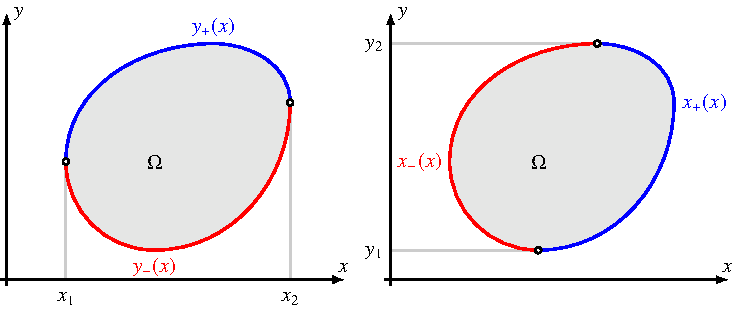
\includegraphics{chapters/040-felder/images/greenbeweis.pdf}
\caption{Beweis des Satzes von Green für ein Gebiet, welches durch
die Graphen zweier Funktionen $y_(x)$ und $y_+(x)$ 
berandet ist.
Alternativ kann das gleiche Gebiet auch durch die Graphen der Funktionen
$x_-(y)$ und $x_+(y)$ berandet werden.
Die Verwendung der beiden Berandungsarten für verschiedene Komponenten
in der Formel von Green ermöglicht den Beweis.
\label{buch:felder:fundamentallemma:fig:greenbeweis}}
\end{figure}

Es genügt damit, den Satz von Green für Gebiete zu beweisen, dessen Rand
aus den Graphen der Funktionen $y_-(x)$ und $y_+(x)$ für den unteren und
oberen Rand und den vertikalen Strecken von $(x_i,y_-(x_i))$ nach
$(x_1,y_+(x_i))$ besteht
(Abbildung~\ref{buch:felder:fundamentallemma:fig:greenbeweis}).

Mit dieser Beschreibung des Gebietes berechnen wir jetzt beide Seiten
von \eqref{buch:felder:fundamentallemma:eqn:green} 
für $g=0$ und zeigen, dass sie gleich sind.
Das Integral des zweiten
Terms des Integranden auf der linken Seite von
\eqref{buch:felder:fundamentallemma:eqn:green} wird zu
\begin{align}
I_l
&=
-\int_{\Omega}
\frac{\partial f}{\partial y}(x,y)
\,dx\,dy
=
-
\int_{x_1}^{x_2}
\int_{y_(x)}^{y_+(x)}
\frac{\partial f}{\partial y}(x,y)
\,dy
\,dx.
\notag
\intertext{Das Integral kann mit dem Hauptsatz der Integralrechung
ausgeführt werden und ergibt}
&=
-
\int_{x_1}^{x_2}
\biggl[ 
f(x,y)
\biggr]_{y_-(x)}^{y_+(x)}
\,dx
=
\int_{x_1}^{x_2}
-f(x,y_+(x))+f(x,y_-(x))
\,dx
\label{buch:felder:fundamentallemma:eqn:greenhaupt}
\end{align}
Die rechte Seite von \eqref{buch:felder:fundamentallemma:eqn:green}
besteht aus vier Teilen, die einzeln berechnet werden können:
\begin{align*}
I_r
&=
\int_{x_1}^{x_2} f(x,y_-(x)),dx
+
\int_{y_-(x_2)}^{y_+(x_2)} \underbrace{g(x,y)}_{\displaystyle=0}\,dy
+
\int_{x_2}^{x_1} f(x,y_+(x))\,dx
+
\int_{y_+(x_1)}^{y_-(x_1)} \underbrace{g(x,y)}_{\displaystyle=0}\,dx
\intertext{Es bleiben nur der erste und dritte Term stehen, die zusammen
das Gleiche ergeben wir $I_l$:}
&=
\int_{x_1}^{x_2} f(x,y_-(x))\,dx
-
\int_{x_1}^{x_2} f(x,y_+(x))\,dx
=
I_l.
\end{align*}
Damit ist die Formel~\eqref{buch:felder:fundamentallemma:eqn:green}
für $g=0$ beweisen.

Um die Formel~\eqref{buch:felder:fundamentallemma:eqn:green} auch
für $f=0$ und $g\ne 0$ zu beweisen, geht man gleich vor mit 
einer Zerlegung des Gebietes in horizontale Streifen.
Da die Formel linear ist in $f$ und $g$ folgt die Behauptung.
\end{proof}

Der entscheidende Schritt im Beweis war die Anwendung des Hauptsatzes
der Integralrechnung in
\eqref{buch:felder:fundamentallemma:eqn:greenhaupt}.
Damit wird auch gerechtfertigt, dass der Satz von Green eine Art
Erweiterung des Hauptsatzes auf zweidimensionale Gebiet ist.

%
% Der Satz von Green in vektorieller Schreibweise
%
\subsubsection{Der Satz von Green in vektorieller Schreibweise}
Die beiden Funktionen $f$ und $g$ im Satz von Green können als
ein dreidimensionales, differenzierbares Vektorfeld
\[
\vec{v}(x,y,z)
=
\begin{pmatrix}
f(x,y)\\
g(x,y)\\
0
\end{pmatrix}
\]
definiert auf der offenen Teilmenge $\Omega\times\mathbb{R}\subset\mathbb{R}^3$.
Der Integrand auf der linken Seite von
\eqref{buch:felder:fundamentallemma:eqn:green} ist die $z$-Komponente
\[
(\operatorname{rot}\vec{v})_z
=
\frac{\partial g}{\partial x}-\frac{\partial f}{\partial y}
\]
der Rotation von $\vec{v}$.
Das Integral auf der linken Seite von
\eqref{buch:felder:fundamentallemma:eqn:green}
ist daher die das Flächenintegral
\[
\int_\Omega
\frac{\partial g}{\partial x}-\frac{\partial f}{\partial y}\,dx\,dy
=
\int_\Omega
\operatorname{rot} \vec{v}
\cdot \,do.
\]
der Rotation über die Fläche $\Omega$ betrachtet als die Einbettung
$\Omega$ in $\mathbb{R}^3$ mittels der Abbildung $(x,y)\mapsto (x,y,0)$.

Die rechte Seite von
\eqref{buch:felder:fundamentallemma:eqn:green} kann mit einer
Parametrisierung $\gamma\colon [a,b]\to \mathbb{R}^3$ 
als das Wegintegral
\begin{align*}
\int_{\partial\Omega} \bigl(f(x,y)\,dx + g(x,y)\,dy\bigr)
&=
\int_a^b
f(\gamma_x(t),\gamma_y(t))\dot{\gamma}_x(x,y)
+
g(\gamma_x(t),\gamma_y(t))\dot{\gamma}_y(x,y)
\,dt
\\
&=
\int_a^b
\begin{pmatrix}
f\circ\gamma(t)\\
g\circ\gamma(t)\\
0
\end{pmatrix}
\cdot
\dot{\gamma}(t)
\,dt
\\
&=
\int_a^b
\vec{v}\circ\gamma(t)
\cdot
\dot{\gamma}(t)
\,dt
\\
&=
\oint \vec{v}\cdot\,ds.
\end{align*}
In dieser Form wird der Satz von Green später in
Satz~\ref{buch:felder:fundamentallemma:satz:stokes} verallgemeinert.

%
% Der Satz von Gauss
%
\subsubsection{Der Satz von Gauss}
%
% 3dimagetemplate.tex
%
% (c) 2021 Prof Dr Andreas Müller, OST Ostschweizer Fachhochschule
%
\documentclass[tikz]{standalone}
\usepackage{times}
\usepackage{amsmath}
\usepackage{txfonts}
\usepackage[utf8]{inputenc}
\usepackage{graphics}
\usetikzlibrary{arrows,intersections,math,calc}
\usepackage{ifthen}
\begin{document}

\newboolean{showgrid}
\setboolean{showgrid}{false}
\def\breite{7}
\def\hoehe{4}

\def\achslabel{
	\node at (-1.75,-1.35) {$x$};
	\node at (1.8,-1.3) {$y$};
	\node at (0.7,1.1) {$z$};
}
\def\marke#1#2#3{
	\fill[color=white,opacity=0.7] ($#1+(-0.6,-0.2)$) rectangle +(1.2,0.4);
	\node[color=#3] at #1 {$#2\mathstrut$};
}
\definecolor{rot}{rgb}{0.8,0.4,0.6}
\definecolor{blau}{rgb}{0.4,0.6,0.8}
\begin{tikzpicture}[>=latex,thick]

% Povray Bild
\begin{scope}[xshift=-4.4cm]
\node at (0,0) {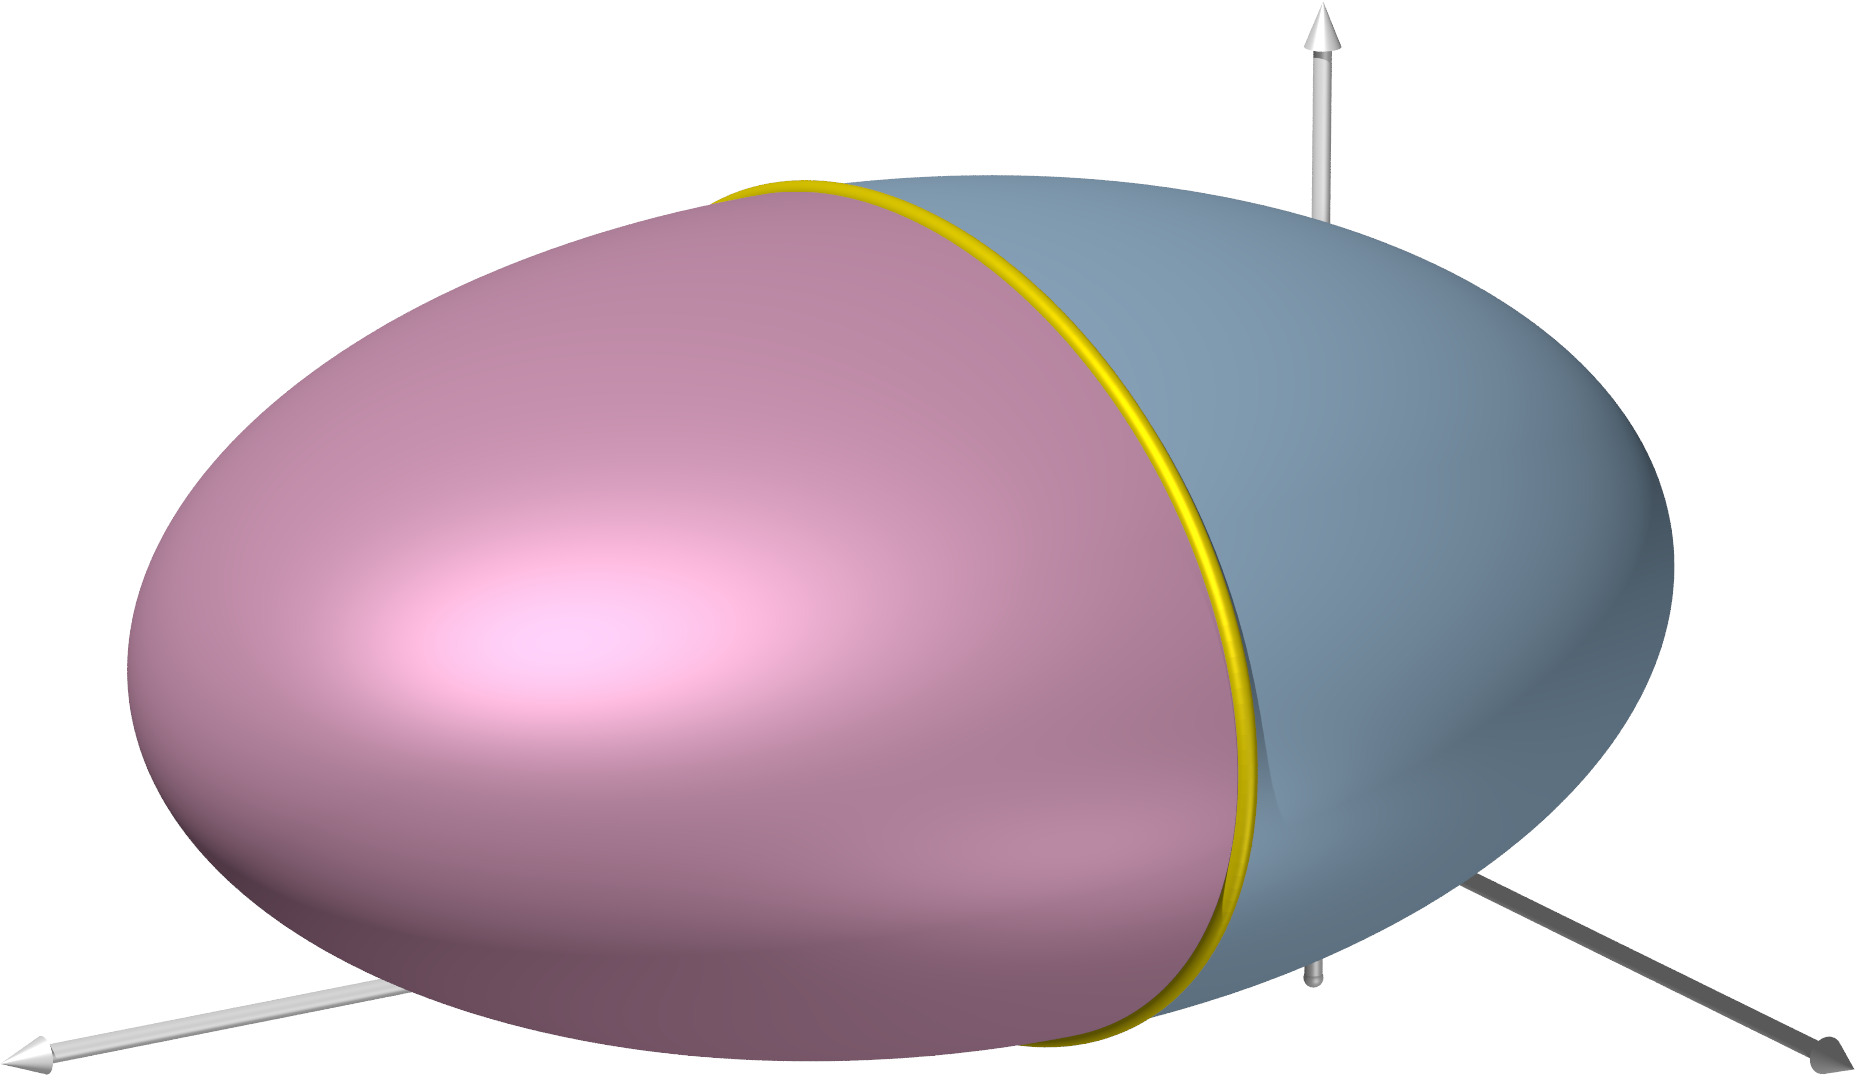
\includegraphics[width=4.2cm]{gaussx.jpg}};
\achslabel
\marke{(-0.7,-0.3)}{x_+(y,z)}{rot}
\marke{(1.4,0.1)}{x_-(y,z)}{blau}
\end{scope}

\begin{scope}
\node at (0,0) {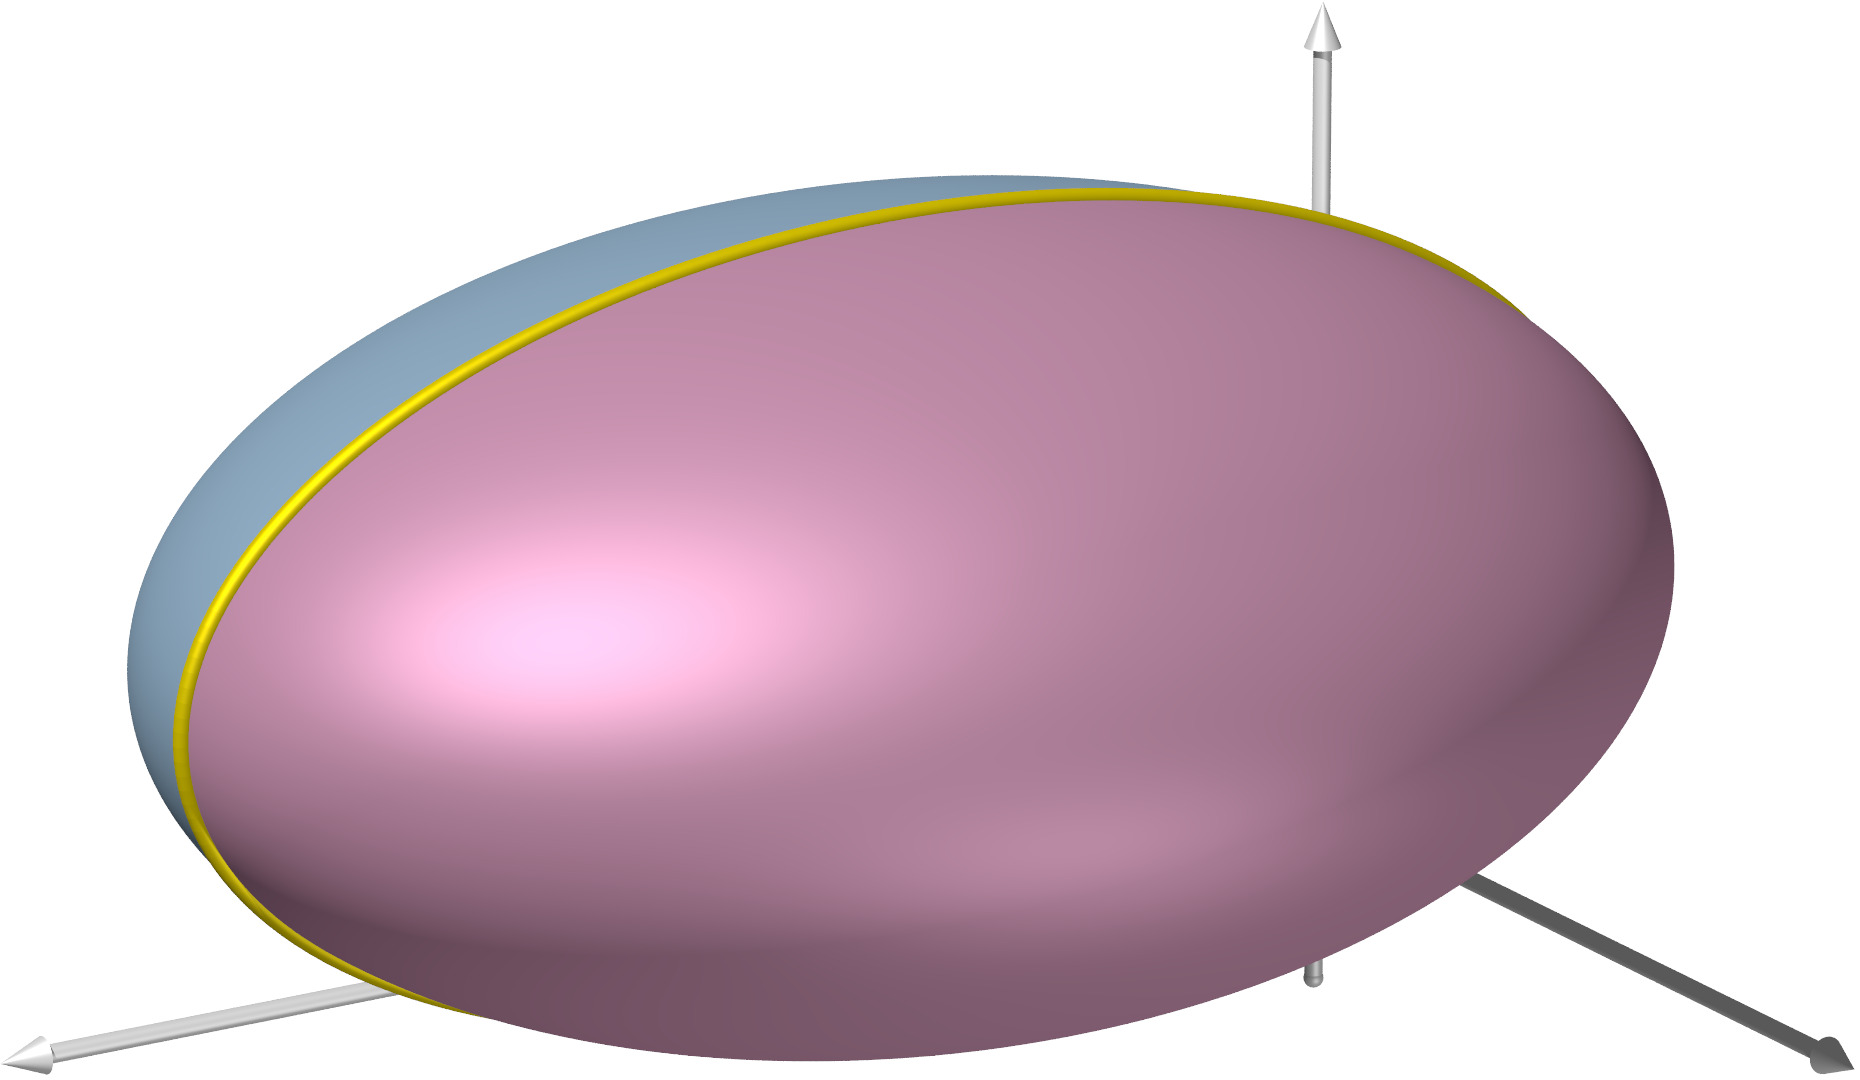
\includegraphics[width=4.2cm]{gaussy.jpg}};
\achslabel
\marke{(0.4,-0.3)}{y_+(x,z)}{rot}
\marke{(-1.4,0.7)}{y_-(x,z)}{blau}
\end{scope}

\begin{scope}[xshift=4.4cm]
\node at (0,0) {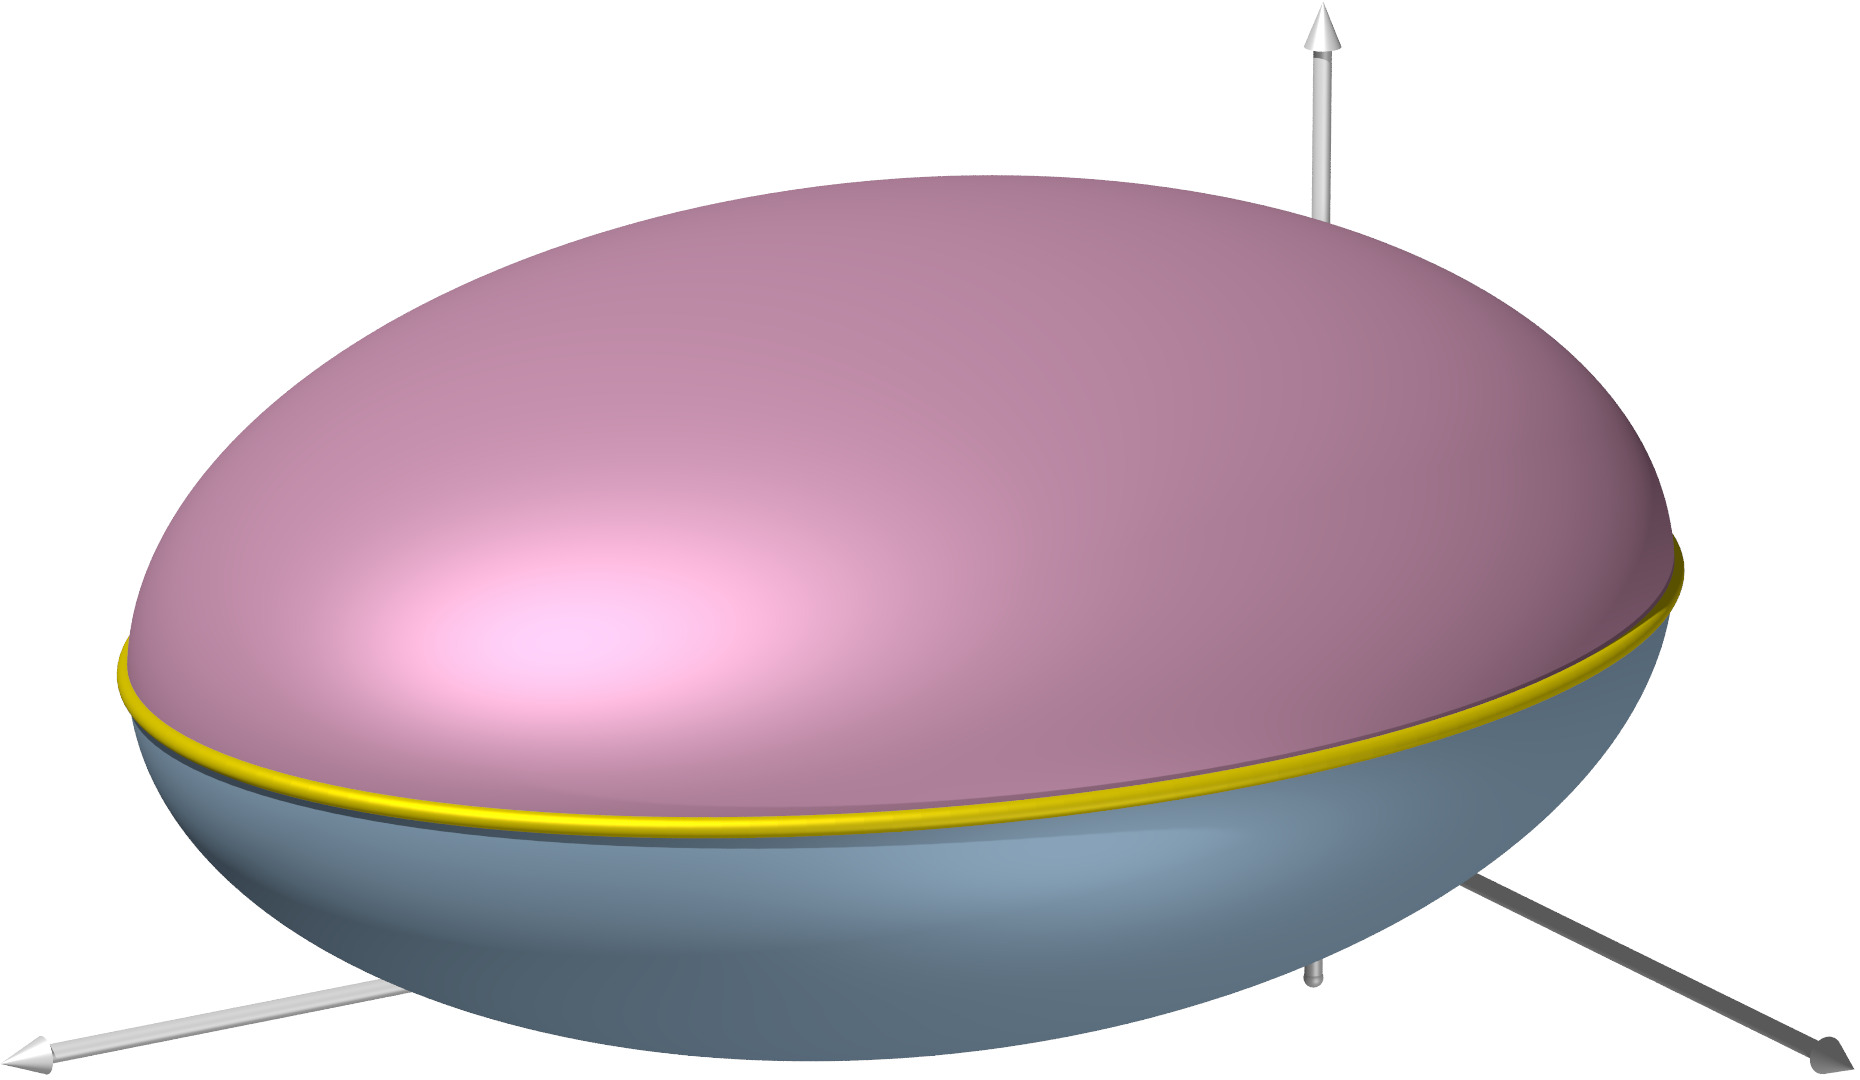
\includegraphics[width=4.2cm]{gaussz.jpg}};
\achslabel
\marke{(0.0,0.3)}{z_+(x,y)}{rot}
\marke{(-0.2,-0.95)}{z_-(x,y)}{blau}
\end{scope}

% Gitter
\ifthenelse{\boolean{showgrid}}{
\draw[step=0.1,line width=0.1pt] (-\breite,-\hoehe) grid (\breite, \hoehe);
\draw[step=0.5,line width=0.4pt] (-\breite,-\hoehe) grid (\breite, \hoehe);
\draw                            (-\breite,-\hoehe) grid (\breite, \hoehe);
\fill (0,0) circle[radius=0.05];
}{}

\end{tikzpicture}

\end{document}


Der Satz~\ref{buch:felder:fundamentallemma:satz:green} von Green
war das erste Beispiel eines Satzes, der ein Gebietsintegral über eine
``abgeleitete Funktion'' in ein Randintegral umzuwandeln gestattet, wobei
die Ableitung wegfällt.
Der Beweis wie auch die Formulierung des Satzes gehen von einer
zweidimensionalen Situation aus und es ist nicht offensichtlich,
wie die Verallgemeinerung auf höhere Dimensionen zu formulieren wäre.
Die Antwort gibt der folgende Satz von Gauss.

\begin{satz}[Gauss]
\label{buch:felder:fundamentallemma:satz:gauss}
\index{Gauss!Satz von}
\index{Satz!von Gauss}
Ist $g(x)$ ein stetig differenzierbares Vektorfeld auf einem Gebiet
$\Omega$ mit glattem Rand $\partial\Omega$ dann gilt
\begin{equation}
\int_\Omega \operatorname{div}g(x)\,dx
=
\int_{\partial\Omega} g(x)\cdot do(x),
\label{buch:felder:fundamentallemma:eqn:gauss}
\end{equation}
wobei das zweite Integral der Fluss des Vektorfeldes $g(x)$ durch
die Randfläche ist.
\end{satz}

\begin{proof}
Der Beweis des Satzes von Green war dadurch erfolgreich, dass für jeden
Term des Integranden eine andere, speziell gut geeignete Zerlegung
des Integrationsgebietes gewählt werden konnte, mit der das Integral
mit Hilfe des Hauptsatzes der Integralrechnung vereinfacht werden konnte.
Diese Vorgehensweise führt auch im vorliegenden Fall zum Erfolg.
Für die Zerlegung der Oberfläche verwenden wir die Parametrisierungen
gemässs Abbildung~\ref{buch:felder:fundamentallemma:fig:gauss}.

Wir zerlegen das Integrationsgebiet in zylindrische ``Säulen'', die
oben und unten durch die Graphen der Funktionen $z_-(x,y)$ und $z_+(x,y)$ 
berandet sind.
Der Grundriss der Säule ist ein 2-dimensionales Gebiet $G$.
Der Rand einer solchen Säule besteht dann zusätzlich noch aus der
Mantelfläche, deren Normale aber überall senkrecht auf dem Standarbasisvektor
$\vec{e}_3$ ist.

Wir im Satz von Green berechnen wir die linke Seite von
\eqref{buch:felder:fundamentallemma:eqn:gauss} für eine Säule und erhalten
\begin{align*}
I_l
&=
\int_\Omega \operatorname{div}g(x)\,dx
=
\int_{G}\int_{z_-(x,y)}^{z_+(x,y)}
\frac{\partial g_3}{\partial z}(x,y,z)
\,dz\,dx\,dy
\\
&=
\int_G \biggl[ g_3(x,y,z)\biggr]_{z_-(x,y)}^{z_+(x,y)}\,dx\,dy
=
\int_G g_3(x,y,z_+(x,y)) - g_3(x,y,z_-(x,y)) \,dx\,dy
\end{align*}
Die rechte Seite ist ein Oberflächenintegral über die drei früher
identifizierten Teile der Oberfläche, wobei der Teil über die Mantelfläche
verschwindet, weil die Normale auf die Mantelfläche senkrecht auf dem
Vektor $g(x,y,z)$ steht.
Es müssen daher nur die Endflächen berücksichtigt werden.
Das Flächenelement auf der Fläche $z(x,y)$ ist 
\[
\renewcommand{\arraystretch}{1.8}
\begin{pmatrix}
1\\
0\\
\displaystyle
\frac{\partial z}{\partial x}
\end{pmatrix}
\times
\begin{pmatrix}
0\\
1\\
\displaystyle
\frac{\partial z}{\partial y}
\end{pmatrix}
\,dx\,dy
=
\begin{pmatrix}
\displaystyle
-\frac{\partial z}{\partial y}\\
\displaystyle
-\frac{\partial z}{\partial x}\\
1
\end{pmatrix}
\,dx\,dy.
\]
Für die untere Endfläche muss die Normale mit dem entgegegengesetzten 
Vorzeichen gewählt werden, damit sie nach aussen zeigt.
Damit wird das Integral über die Endflächen
\begin{align*}
I_r
&=
\int_{\partial\Omega} g(x) \cdot do(x)
=
\int_{G} g_3(x,y,z_+(x,y)) \,dx\,dy
-
\int_{G} g_3(x,y,z_-(x,y)) \,dx\,dy.
\end{align*}
Dies stimmt mit $I_l$ überein, was den Satz von Gauss für ein
Vektorfeld mit $g_1(x,y)=g_2(x,y)=0$ beschreibt.

Indem man Zylinder mit Achsenrichtungen parallel zu anderen
Koordinatenrichtungen verwendet, kann man den Satz von Gauss auch für
jede andere Komponente des Vektorfeldes $g(x)$ beweisen.
Da die Formel~\eqref{buch:felder:fundamentallemma:eqn:gauss} 
linear in $g(x)$ ist, folgt die allgemeine Formel.
\end{proof}

Der Satz von Gauss gilt noch etwas allgemeiner auch für Integrale der
Divergenz eines $n$-dimensionalen differenzierbaren Vektorfeldes über
ein $n$-dimensionales Gebiet.
Der Beweis bleibt ist mutatis mutandis auch auf die allgemeinere Situation
anwendbar.

Der Satz von Gauss ermöglicht also, einen Divergenz-Operator loszuwerden,
indem man zu einem Integral über den Rand übergeht.

%
% Partielle Integration und der Satz von Gauss
%
\subsubsection{Partielle Integration und der Satz von Gauss}
Die partielle Integrationsformel für Funktionen einer Variablen folgt aus
der Formel für die Ableitung eines Produktes von Funktionen.
Wir erwarten daher eine ähnliche Formel für die Ableitung von
Funktionen mehrere Variablen, wir müssen jedoch jeweils den richtigen
Differentialoperator wählen.

Auf ein Vektorfeld ist der Divergenzoperator anwendbar, für eine
differenzierbare skalare Funktion $f\colon\mathbb{R}^n\to\mathbb{R}$
und ein differenzierbares $n$-dimensionales Vektorfeld
$g\colon\mathbb{R}^n\to\mathbb{R}^n$ gilt die Produktregel
\[
\operatorname{div}(fg)
=
(\grad f)g
+
f\operatorname{div}g
\qquad\Rightarrow\qquad
\left\{
\begin{aligned}
(\grad f)g &= \operatorname{div}(fg) - f\operatorname{div}g \\
f\operatorname{div}g &= \operatorname{div}(fg) - (\grad f)g
\end{aligned}
\right.
\]
Integrieren wir die Formen auf der rechten Seite über ein Gebiet $\Omega$
und wenden den Satz~\ref{buch:felder:fundamentallemma:satz:gauss}
von Gauss auf auf den Term $\operatorname{div}(fg)$ an, folgt im
ersten Fall die Identität
\begin{align*}
\int_{\Omega} (\grad f)(x) g(x)\,dx
&=
\int_{\partial\Omega} f(x)g(x)\cdot do(x)
-
\int_{\Omega} f(x)\operatorname{div}g(x)\,dx.
\end{align*}

\begin{satz}[partielle Integration für Vektorfelder]
Sei $f\colon\mathbb{R}^n\to\mathbb{R}$ eine differenzierbare Funktion,
$g\colon\mathbb{R}^n\to\mathbb{R}^n$ ein differenzierbares
$n$-dimensionales Vektorfeld und $\Omega$ ein Gebiet mit stückweise
glattem Rand.
Dann gilt
\begin{align*}
\int_{\Omega} (\grad f)(x) g(x)\,dx
&=
\int_{\partial\Omega} f(x)g(x)\cdot do(x)
-
\int_{\Omega} f(x)\operatorname{div}g(x)\,dx.
\\
\int_{\Omega} (\nabla f)(x)g(x)\,dx
&=
\int_{\partial\Omega} f(x)g(x)\cdot do(x)
-
\int_{\Omega} f(x)\nabla\cdot g(x)\,dx.
\qedhere
\end{align*}
\end{satz}

Die partielle Integration verschiebt den Differentialoperator $\nabla$
vom Faktor $f$ auf den Faktor $g$, dabei tritt ein zusätzlicher Term
auf, der nur von den Werten der Funktionen auf dem Rand abhängt.


%
% Der Satz von Stokes
%
\subsubsection{Der Satz von Stokes}
Die vektorielle Schreibweise des Satzes von Green zeigt bereits,
wie er sich auf die dreidimensionale Situation verallgemeinert werden kann.

\begin{satz}[Stokes]
\label{buch:felder:fundamentallemma:satz:stokes}
\index{Satz!von Stokes}%
\index{Stokes!Satz von}%
Sei $g(x)$ ein stetig differenzierbares, dreidimensionales Vektorfeld
und $S$ eine zweidimensionale Fläche, die von der geschlossenen
Kurve $\partial S$ berandet ist.
Dann gilt
\begin{equation}
\int_S \operatorname{rot} g(x)\,do(x)
=
\oint_{\partial S} g(x)\cdot ds,
\label{buch:felder:fundamentallemma:eqn:stokes}
\end{equation}
wobei das erste Integral der Fluss des Vektorfeldes $\operatorname{rot}g$
durch die Fläche $S$ und das zweite Integral des Pfadintegral des
Vektorfeldes entlang der Randkurve ist.
\end{satz}

\begin{proof}
Wir beweisen den Satz von Stokes für eine geeignete Parametrisierung
der Fläche $S$.
Sei also $\Omega$ ein Gebiet in $\mathbb{R}^2$ und 
$\varphi\colon\overline{\Omega}\to\mathbb{R}^3$ eine Parametrisierung
der Fläche $S$.
Sei ausserdem $\gamma\colon[a,b]\to\mathbb{R}^2$ eine Parametrisierung
des Randes von $\Omega$, so dass $\varphi\circ\gamma$ eine Parametrisierung
des Randes $\partial S$ von $S$ ist.
Mit Hilfe der Parametrisierung $\varphi$ können jetzt die Integrale
im Satz von Stokes auf die zweidimensionale Situation des Satzes von
Green zurückgeführt werden.

Das Integral über den Rand von $S$ bekommt die Form
\begin{align*}
\int_{\partial S}g\cdot\,ds
&=
\int_a^b
g\circ\varphi(\gamma(t))
\cdot
\biggl(
\frac{\partial\varphi}{\partial u}
\dot{\gamma}_u(t)
+
\frac{\partial\varphi}{\partial v}
\dot{\gamma}_u(t)
\biggr)
\,dt
\\
&=
\int_a^b
\biggl(
\underbrace{
g(\varphi(\gamma(t)))
\cdot
\frac{\partial\varphi}{\partial u}
}_{\displaystyle P}
\biggr)
\dot{\gamma}_u(t)
+
\biggl(
\underbrace{
g(\varphi(\gamma(t)))
\cdot
\frac{\partial\varphi}{\partial v}
}_{\displaystyle Q}
\biggr)
\dot{\gamma}_v(t)
\,dt
.
\end{align*}
Die Funktionen $P$ und $Q$ sind die beiden Funktionen, auf die
der Satz von Green angewendet werden soll.

Der Satz von Green sagt über die beiden Funktionen $P$ und $Q$,
dass die rechte Seite von~\eqref{buch:felder:fundamentallemma:eqn:stokes}
mit
\begin{equation}
\int_\Omega
\frac{\partial Q}{\partial u}
-
\frac{\partial P}{\partial v}
\,du\,dv
\label{buch:felder:fundamentallemma:eqn:stokesintegrand}
\end{equation}
übereinstimmt.
Es müssen jetzt also die Ableitungen $P$ und $Q$ nach $u$ und $v$
berechnet werden, sie sind
\begin{align*}
\frac{\partial Q}{\partial u}
&=
\frac{\partial g\circ\varphi}{\partial u}
\cdot
\frac{\partial\varphi}{\partial v}
+
g\circ\varphi
\cdot
\frac{\partial^2 \varphi}{\partial u\,\partial v}
\\
\frac{\partial P}{\partial v}
&=
\frac{\partial g\circ\varphi}{\partial v}
\cdot
\frac{\partial \varphi}{\partial u}
+
g\circ\varphi
\cdot
\frac{\partial^2\varphi}{\partial v\,\partial u}
\end{align*}
Da $\varphi$ stetig differenzierbar ist, stimmen die zweiten Terme auf
der rechten Seite überein und verschwinden daher im Integranden
\begin{align}
\frac{\partial Q}{\partial u}
-
\frac{\partial P}{\partial v}
&=
\frac{\partial g\circ\varphi}{\partial u}
\cdot
\frac{\partial\varphi}{\partial v}
-
\frac{\partial g\circ\varphi}{\partial v}
\cdot
\frac{\partial \varphi}{\partial u}
\notag
\intertext{von \eqref{buch:felder:fundamentallemma:eqn:stokesintegrand}.
Wir schreiben das Skalarprodukt mit Hilfe der Transposition und erhalten
}
&=
\biggl(\frac{\partial\varphi}{\partial v}\biggr)^t
\frac{\partial g\circ\varphi}{\partial u}
-
\biggl(\frac{\partial \varphi}{\partial u}\biggr)^t
\frac{\partial g\circ\varphi}{\partial v}
\notag
\intertext{und wenden die Kettenregel auf $g\circ\varphi$ an, so entsteht}
&=
\biggl(\frac{\partial\varphi}{\partial v}\biggr)^t
Dg
\frac{\partial\varphi}{\partial u}
-
\biggl(\frac{\partial\varphi}{\partial u}\biggr)^t
Dg
\frac{\partial\varphi}{\partial v}
\notag
\\
&=
\biggl(\frac{\partial\varphi}{\partial v}\biggr)^t
(
Dg
-
Dg^t
)
\frac{\partial\varphi}{\partial u}.
\label{buch:felder:fundamentallemma:eqn:produkt}
\end{align}
Die Matrix in Klammern auf der rechten Seite ist
\begin{align*}
Dg-Dg^t
&=
\renewcommand{\arraystretch}{1.8}
\begin{pmatrix}
\displaystyle \frac{\partial g_1}{\partial x_1}
	&\displaystyle \frac{\partial g_1}{\partial x_2}
		&\displaystyle \frac{\partial g_1}{\partial x_3}
\\
\displaystyle \frac{\partial g_2}{\partial x_1}
	&\displaystyle \frac{\partial g_2}{\partial x_2}
		&\displaystyle \frac{\partial g_2}{\partial x_3}
\\
\displaystyle \frac{\partial g_3}{\partial x_1}
	&\displaystyle \frac{\partial g_3}{\partial x_2}
		&\displaystyle \frac{\partial g_3}{\partial x_3}
\end{pmatrix}
-
\begin{pmatrix}
\displaystyle\frac{\partial g_1}{\partial x_1}
	&\displaystyle\frac{\partial g_2}{\partial x_1}
		&\displaystyle\frac{\partial g_3}{\partial x_1}
\\
\displaystyle\frac{\partial g_1}{\partial x_2}
	&\displaystyle\frac{\partial g_2}{\partial x_2}
		&\displaystyle\frac{\partial g_3}{\partial x_2}
\\
\displaystyle\frac{\partial g_1}{\partial x_3}
	&\displaystyle\frac{\partial g_2}{\partial x_3}
		&\displaystyle\frac{\partial g_3}{\partial x_3}
\end{pmatrix}
\\
&=
\renewcommand{\arraystretch}{1.8}
\begin{pmatrix}
0
&\displaystyle
\frac{\partial g_1}{\partial x_2}-\frac{\partial g_2}{\partial x_1}
&\displaystyle
\frac{\partial g_1}{\partial x_3}-\frac{\partial g_3}{\partial x_1}
\\
\displaystyle
\frac{\partial g_2}{\partial x_1}-\frac{\partial g_1}{\partial x_2}
&0
&\displaystyle
\frac{\partial g_2}{\partial x_3}-\frac{\partial g_3}{\partial x_2}
\\
\displaystyle
\frac{\partial g_3}{\partial x_1}-\frac{\partial g_1}{\partial x_3}
&\displaystyle
\frac{\partial g_3}{\partial x_2}-\frac{\partial g_2}{\partial x_3}
&0
\end{pmatrix}
\\
&=
\begin{pmatrix}
0
	&(\operatorname{rot} g)_3
		&-(\operatorname{rot} g)_2
\\
-(\operatorname{rot}g)_3
	&0
		&(\operatorname{rot}g)_1
\\
(\operatorname{rot}g)_2
	&-(\operatorname{rot}g)_1
		&0
\end{pmatrix}.
\end{align*}
Damit kann man jetzt auch das Produkt
\begin{align*}
\biggl(\frac{\partial\varphi}{\partial v}\biggr)^t
(
Dg
-
Dg^t
)
\frac{\partial\varphi}{\partial u}
&=
\begin{pmatrix}
\displaystyle
\frac{\partial \varphi_1}{\partial v}&
\displaystyle
\frac{\partial \varphi_2}{\partial v}&
\displaystyle
\frac{\partial \varphi_3}{\partial v}
\end{pmatrix}
{\renewcommand{\arraystretch}{2.0}
\begin{pmatrix}
\displaystyle
(\operatorname{rot}g)_3 \frac{\partial\varphi_2}{\partial u}
-
(\operatorname{rot}g)_2 \frac{\partial\varphi_3}{\partial u}
\\
\displaystyle
(\operatorname{rot}g)_1 \frac{\partial\varphi_3}{\partial u}
-
(\operatorname{rot}g)_3 \frac{\partial\varphi_1}{\partial u}
\\
\displaystyle
(\operatorname{rot}g)_2 \frac{\partial\varphi_1}{\partial u}
-
(\operatorname{rot}g)_1 \frac{\partial\varphi_2}{\partial u}
\end{pmatrix}}
\\
&=
(\operatorname{rot}g)_1
\biggl(
\frac{\partial\varphi_3}{\partial u}
\frac{\partial\varphi_2}{\partial v}
-
\frac{\partial\varphi_2}{\partial u}
\frac{\partial\varphi_3}{\partial v}
\biggr)
+
(\operatorname{rot}g)_2
\biggl(
\frac{\partial\varphi_1}{\partial u}
\frac{\partial\varphi_3}{\partial v}
-
\frac{\partial\varphi_3}{\partial u}
\frac{\partial\varphi_1}{\partial v}
\biggr)
\\
&\qquad
+
(\operatorname{rot}g)_3
\biggl(
\frac{\partial\varphi_2}{\partial u}
\frac{\partial\varphi_1}{\partial v}
-
\frac{\partial\varphi_1}{\partial u}
\frac{\partial\varphi_2}{\partial v}
\biggr)
\\
&=
\operatorname{rot}g\cdot
\biggl(
\frac{\partial\varphi}{\partial u}
\times
\frac{\partial\varphi}{\partial v}
\biggr)
\end{align*}
berechnen.
Das Integral des Satzes von Green über $\Omega$ ist jetzt
\begin{align*}
\int_{\partial S} g\cdot ds
&=
\int_\Omega
\operatorname{rot}g
\cdot
\biggl(
\frac{\partial\varphi}{\partial u}
\times
\frac{\partial\varphi}{\partial v}
\biggr)\,dx\,dy
\\
&=
\int_S
\operatorname{rot} g
\cdot
do.
\end{align*}
Dies ist der Satz von Stokes bewiesen.
\end{proof}

%
% Partielle Integration und der Satz von Stokes
%
\subsubsection{Partielle Integration und der Satz von Stokes}
Für eine differenzierbare skalare Funktion
$f\colon\mathbb{R}^3\to\mathbb{R}$, ein differenzierbares dreidimensionales
Vektorfeld $g\colon\mathbb{R}^3\to\mathbb{R}^3$.
Dann gilt die Produktregel
\[
\operatorname{rot}(f g)
=
(\grad f)\times g
+
f\operatorname{rot}g
\qquad\Rightarrow\qquad
(\grad f)\times g
=
\operatorname{rot}(fg)
-
f\operatorname{rot}g.
\]
Integration über die Fläche $S\subset \mathbb{R}^3$, die von einer
geschlossenen Kurve berandet ist, ermöglicht auf den mittleren
Term den Satz von Stokes anzuwenden, so entsteht die Identität
\begin{align*}
\int_{S}(\grad f)(x)\times g(x) \cdot do(x)
&=
\int_{\partial S} f(x)g(x)\cdot ds(x)
-
\int_{S} f(x)\operatorname{rot}g(x)\cdot do(x)
\intertext{oder in der Schreibweise mit dem Nabla-Operator}
\int_{S}(\nabla f)(x)\times g(x) \cdot do(x)
&=
\int_{\partial S} f(x)g(x)\cdot ds(x)
-
\int_{S} f(x)(\nabla\times g)(x)\cdot do(x).
\end{align*}
Wieder kann der Differentialoperator vom einen Faktor auf den anderen
zu verschieben.
Dabei entsteht wieder ein Term, der nur von den Funktionswerten
auf dem Rand der Fläche $S$ abhängt.



